\chapter{Conclusioni}
\label{chap:Capitolo1}

Durante lo studio di fattibilitá e il successivo sviluppo, abbiamo constatato che le potenzialità del Dial in ambito industriale sono molteplici, dal miglioramento della User Experience alla precisione adottata nell’utilizzo.
Grazie al DialService è stato possibile trasferirle anche in ambito web, in quanto all’interno dell’impresa Loccioni sono presenti moltissimi settori in cui il Dial migliorerebbe molto l’esperienza utente e porterebbe una diminuzione di tempi e costi.
Al momento dello sviluppo, la necessitá di dover passare per un applicazione UWP rappresenta sicuramente una limitazione che andrá tolta qualora il progetto verrá rilasciato in maniera industriale.
A favore di questa critica, nel mese passato, la Google stessa ha rilasciato in fase di Preview una libreria Web chiamata Trial for WebHID, la quale permetterá di far comunicare direttamente con la pagina Web i dispositivi che utilizzano il protocollo HID, come il Dial, permettendo agli sviluppatori futuri di non dover necessariamente passare attraverso una WebView o una applicazione nativa per quel dispositivo.

\begin{figure}[htpb!]
  \centering
  \includegraphics[width=0.2\textwidth]{Potenziometri}
  \caption{Potenziometro utilizzato attualmente}
\end{figure}
Nel nostro caso, l’utilizzo finale del Dial nei banchi prova del gruppo Loccioni, comporterebbe una maggior sicurezza in termini di precisione nella variazione di dati, in quanto al momento vengono utilizzati dei semplici potenziometri con le evidenti limitazione che essi comportano, come ad esempio la presenza di un inizio e fine corsa del potenziometro stesso, l’assenza di feedback durante l’utilizzo, la limitata corsa e di conseguenza la necessaria approssimazione dei singoli step eseguiti.

\begin{figure}[htpb!]
  \centering
  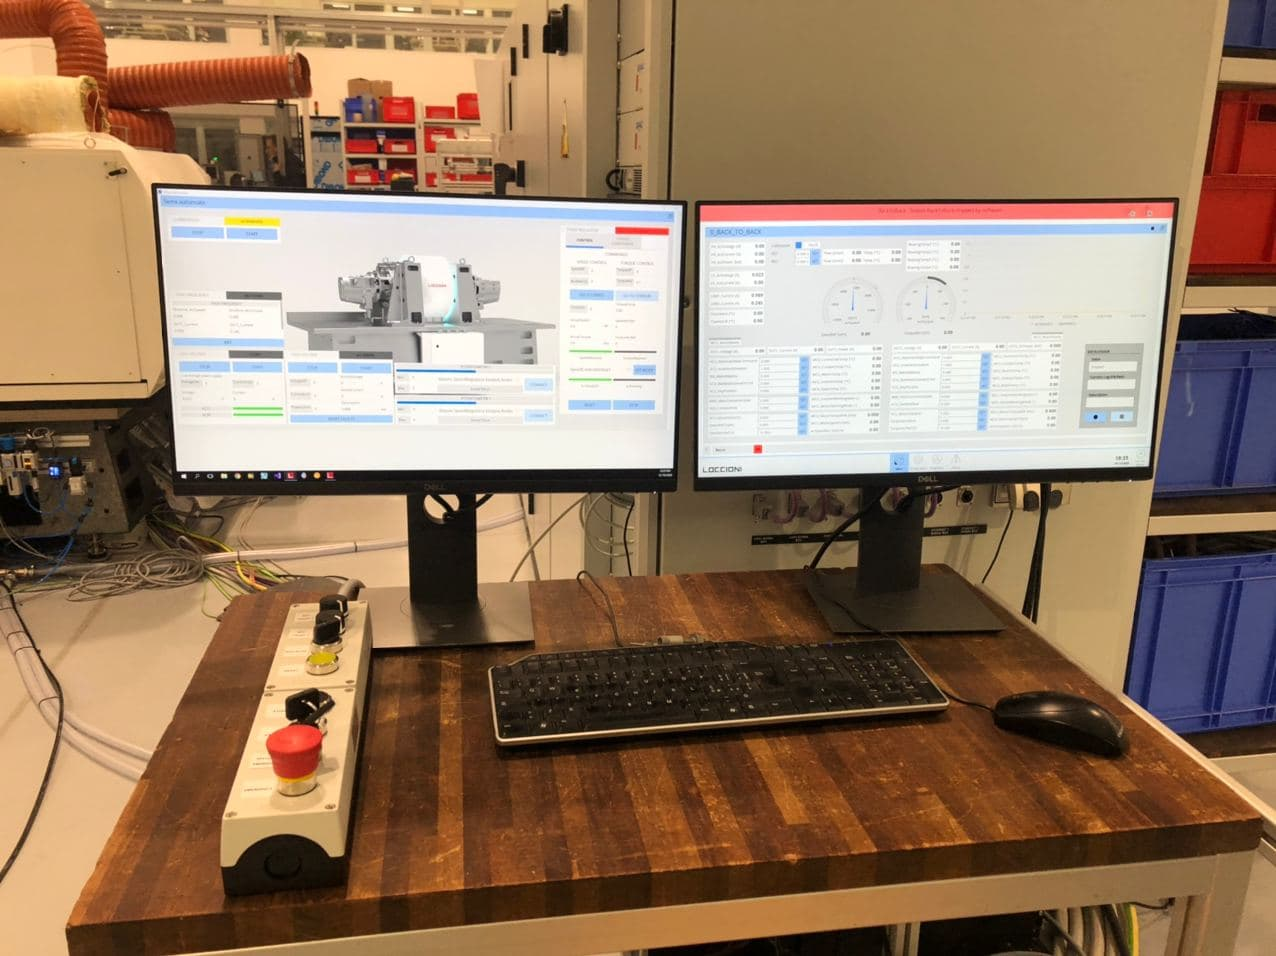
\includegraphics[width=0.2\textwidth]{Postazione}
  \caption{Potenziometro utilizzato attualmente}
\end{figure}

Queste problematiche verrebbero risolte attraverso il Dial, in quanto presenta una “corsa” illimitata, un feedback atpico personalizzabile in base alle operazioni che si svolgono, una precisione laser a 3600 punti e la possibilitá di interagire direttamente con lo schermo, appoggiando il Dial su di esso, permettendo quindi una serie di combinazioni di utilizzo estremamente vasta.